\documentclass[a4paper,12pt, english]{article}
\usepackage[T1]{fontenc}
\usepackage[utf8]{inputenc}
\usepackage{graphicx}
\usepackage{babel}
\usepackage{amsmath}
\usepackage{ulem}
\usepackage{a4wide}
\usepackage{float}

\usepackage{listings}
\usepackage{tabularx}
\usepackage{tabulary}

\usepackage{caption}
\usepackage{subcaption}

\begin{document}

\begin{titlepage}
\begin{center}
\textsc{\Large Computational Physics, Project 5}\\[0.5cm]
\textsc{Candidate number}\\[0.5cm]

\end{center}
\end{titlepage}

\begin{abstract}
In this project we consider Newtonian dynamics for both a two-body and N-body system. For the two-body system we use the Runge-Kutta 4 and the Leap-Frog method, and find that the Leap-Frog method is best for our use when we want long term stability. We simulate a cold collapse of a cluster composed of uniformly distributed particles within a sphere. Since the particles have no relative motion with respect to each other initially, the cluster collapses by gravity. We find that the development of the system after the collapse is highly dependent on whether we add a modification to the Newtonian force to deal with the close distance interaction between the particles. Without this modification the particles attains high kinetic energy, and are spread out after the collapse. With the modification some of the particles will be bound after the collapse, and we will reach an equilibrium state for the cluster.    
\end{abstract}

\section*{$N$-body simulation of an open galactic cluster}

\subsection*{Introduction}

Throughout this project we will develop a code to perform simulations of an open cluster using Newtonian gravity. We will consider the evolution by following the motion of its constituent stars. This interacting classical system require integrating Newton's equation of motion over a long period of time starting from some initial conditions. This type of simulations are called "N-body" simulations.

First we will compare the stability of two different methods for solving differential equations; the fourth order Runge-Kutta and the Leap-Frog method. When we are looking at a system with a large number of particles we are more interested in the statistical properties than the individual motion of each of the particles. This means that the stability of the solution method is more important than its short term accuracy.

First we implement the Newtonian two-body problem in three-dimensions. We choose to look at a hypothetical solar system, with only one planet, the Earth, orbiting the Sun. We will check the stability of the two numerical methods for different time steps and time scales.

Thereafter we will adapt our code to simulate a simple model of how an open cluster is made from the gravitational collapse and interaction among a large number of stars. In this simulation we will assume what is called a "cold collapse", that is that the particles starts with little or no initial velocity. We will rewrite the code so that it works for an arbitrary number of particles. We will start with a uniform (random) distribution within a sphere of a given radius $R_0$. The masses of the particles will be randomly distributed by a Gaussian distribution around ten solar masses with a standard deviation of one solar mass. From our simulations we will extract information about the systems energies. We will look at energy conservation and the ejected particles and their associated energies for a different number of particles $N$.
To take care of the numerical instability that arises when the particles come very close, we will insert a smoothing function.


\subsection*{Theory}

The only force in this problem is gravity, given by Newton's law of gravitation. The force between two objects with masses $M_1$ and $M_2$ is

\[
F = \frac{GM_1 M_2}{r^2}
\]

where $r$ is the distance between them and $G$ the gravitational constant.

In one dimension Newton's second law yields this second-order differential equation

$$m\frac{d^2x}{dt^2} = F(x,t)$$

We can rewrite the second-order ordinary differential equation as a set of coupled first order differential equations.
We know that the velocity and the acceleration is connected to the position by the time derivative so that

\[
\frac{dx}{dt} = v(x,t) \hspace{1cm}\mathrm{and}\hspace{1cm}
\frac{dv_x}{dt} = \frac{F(x,t)}{M} = a(x,t)
\]

Performing a Taylor expansion we get
\[
x(t+h) = x(t) + hx^{(1)} + \frac{h^2}{2}x^{(2)}(t) + O(h^3)
\]

To calculate the next time step of the system we will use two methods for numerically integrating differential equations; the Runga-Kutta method and the Leap-Frog method.

We implement these methods for a Newtonian two-body system, looking at the Earth's orbit around the Sun. In our simulation we assume that the Sun and the Earth is the only objects in the system, and choose the initial conditions such that the orbit of the Earth should be circular.

For circular motion we know that the force must obey the following relation
$$\frac{M_{Earth}v^2}{r} = F_G = \frac{GM_{sun}M_{Earth}}{r^2}$$ where $v$ is the velocity of the Earth.
For circular orbit the velocity of the Earth is $v = \frac{2 \pi r}{1 year}$, where the distance between Sun and Earth is $r = 1 AU$. Hence $v = 2 \pi (AU/years)$. Rearranging the equation we find
$$v^2r = GM_{sun} = 4 \pi ^2 AU^3/years^2$$

We know that for circular motion the velocity will be tangential. It follows that if we choose the initial conditions $ x = 1 AU $ and $ y = 0$, with velocities $v_x = 0$ and $v_y = v_{tangential} = 2 \pi AU/year$ we will get circular orbit.

The next task in the project was to build a model of an open cluster. An open cluster is a group up to a few thousand gravitationally bound stars created from the collapse of a molecular cloud. In our model we work with a few hundred particles. We start the particles with no initial velocity, that is we simulate a so-called "cold collapse". Since the objects have no relative motion with respect to each other initially, the cluster collapses by its gravity.

Since the distribution of the clumps in the cluster is spherical and uniform, all the clumps will collapse simultaneously.
In a system like this the evolution of the system leads to a singularity after a finite time as $N -> \infty$, since all the mass arrives at the origin after a time $\tau_{crunch}$. The time of the collapse is given by $$\tau_{crunch} = \sqrt{\frac{3 \pi}{32G \rho_0}},$$ where $\rho_0$ is the initial mass density.

Our numerical simulation has a finite number of particles $N$, and thus the singularity does not occur. Even if we had the ability to make the simulation for an infinite number of particles, we have approximated the objects as point particles. In the limit where $N -> \infty$, and keeping $\rho_0$ constant, we should get a continuous fluid. However, looking at the particles as point particles, we will not get the uniformly distributed "lump" of mass which leads to the system collapse into a singularity.

Using $\tau_{crunch}$ as an unit of time, we can find $G$ in these units.

\[
\tau_{crunch} = \sqrt{\frac{3 \pi}{32 G \rho_0}} = 1
\]

which gives

\[
\frac{3 \pi}{32G \rho_0} = 1 \hspace{1mm} \Rightarrow \hspace{1mm} G = \frac{3 \pi}{32 \rho_0}
\]

We have that
\[
\rho_0 = \frac{\Sigma M}{V} = \frac{\mu N}{ \frac{4}{3} \pi R_0^3}
\]

where we have used that the total mass is the average mass of the particles, $/mu$, times the number of particle, $N$.

We thus have
\[
G = \frac{3 \pi}{32} \frac{4 \pi R_0^3}{3 \mu N} = \frac{\pi^2 R_0^ 3}{8 \mu N}
\]

When two of the particles come very close we will find that a time step that is reasonable for larger distances now is far too large for our calculations. This because we will get very large accelerations when the particles have close encounters, and thus the necessity for very small time steps. To take care of this numerical instability we introduce a smoothing function. We modify the Newtonian force to make it finite at short ranges
\[
F_{mod} = - \frac{GM_1M_2}{r^2 + \epsilon^2}
\]

The parameter $\epsilon$ is a small real constant which we set to be $\epsilon = 0.15 ly$. We see that setting $\epsilon = 0$ will give us back the standard Newtonian equation of motion. We can justify the correction to the pure Newtonian force by noting that our particles do not represent actual point particles but rather mass distribution of some finite extent.

With this modified force the code does not integrate accurately trajectories in which particles have close encounters, but on a macroscopic scale this trajectories does not play any significant role.


With this modification in place we will look at the particles that are bound. The particles that are ejected will have larger kinetic than potential energy, and thus our bound particles are the ones with a total energy less than zero. For these particles we will find the distribution of potential and kinetic energy. We will check if our results are in agreement with the virial theorem that states that for a bound gravitational system in equilibrium we have
\[
2\langle K\rangle = -\langle V \rangle
\]

To find the potential energy for one particle, we sum over the gravitational force working on it from all the other particles. If we take the sum over the potential energy of all the particles, we get the contribution from the gravitational force twice. Thus the potential energy contribution to the total energy is half of the sum over the potential energy for each particle.
To find the total energy of the system we thus sum over the kinetic energy and half the potential energy of all the particles. In addition we have to subtract the potential energy of the ejected particles, so all effect from these particles is disregarded in our equilibrium system.

We also wish to plot the radial density of the particles in the equilibrium state. To extract the information needed from our simulations, we first find the mass and position of all bound particles. From this we can calculate the center of mass, summing over the mass and position of each particle and dividing by the total mass.


$$ x_{cm} = \frac{1}{M_{tot}} \Sigma M_i x_i $$
$$ y_{cm} = \frac{1}{M_{tot}} \Sigma M_i y_i $$
$$ z_{cm} = \frac{1}{M_{tot}} \Sigma M_i z_i $$

We find the radius of the bound particles relative to the center of mass
\[
r_i = \sqrt{(x_i - x_{cm})^2 + (y_i - y_{cm})^2 + (z_i - z_{cm})^2 }
\]

We then have a sphere centred around the center of mass with particles placed in different distances around it. To find the radial density we can divide the sphere into difference shells. The density of each shell will then be the number of particles within this shell, that is particles in a distance $r_{i-1}$ to $r_i$, divided by the volume of the shell. The volume of each shell will be given by the volume of a sphere with the outer radius subtracted by the volume of a sphere with the inner radius.

\[
d(r_{shell}) = \frac{q}{ \frac{4}{3} \pi r_i^3 - \frac{4}{3} \pi r_{i-1}^3}
\]
 
where $q$ is the number of particles within the shell.

\begin{figure}
        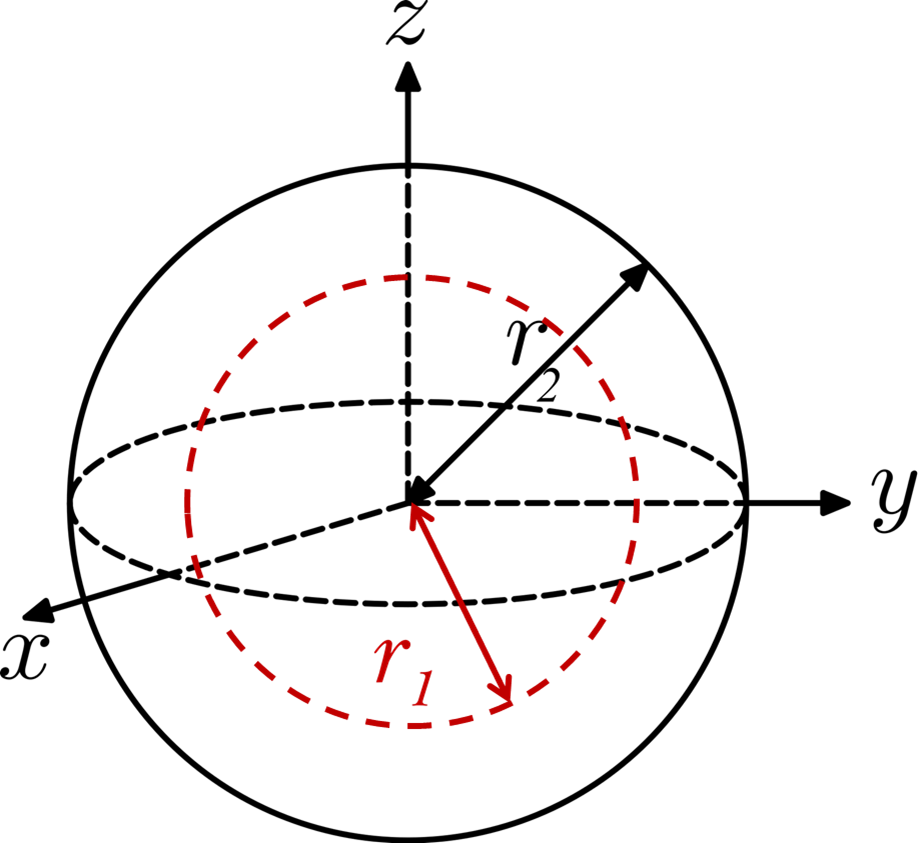
\includegraphics[scale=0.5]{sphere.png}
        \caption{\textit{Illustration from $ http://en.wikipedia.org/wiki/List_of_moments_of_inertia$}}
        \label{fig:sphere}
\end{figure}
        

The radial distribution of particles in this kind of collapse can often be fit very well with the simple expression
\[
n(r) = \frac{n_0}{\left(1 +\left(\frac{r}{r_0}\right)^4\right)}.
\]

 
\subsection*{Method}

Both the Runge-Kutta and the Leap-Frog solvers are methods that advances the solution from $x(t)$ to $x(t+h) = x(t) + hv(t)$ where $h$ is the step length to the new point we are calculating. The step is defined by splitting an interval of size $N$ into sub-intervals $h = \frac{b-a}{N}$. With this step and the derivative of $x$ we can construct the next value of the function.

If we were only to use the derivative at the beginning of each interval when calculating the next step, as in Euler's method, the local truncation error would be on the order of $O(\Delta t^2)$. The Runge-Kutta methods improves the approximation by using trial steps within each interval to make a better estimate of the derivative. The fourth-order Runge-Kutta (RK4) method requires four evaluations in each interval $\Delta t$, and thus reduces the local error to the order of $O(\Delta t^5)$.

 
\subsubsection*{The Runge-Kutta 4 method}

The Runge-Kutta solvers are a set of methods for solving ordinary differential equations for which we know the initial values. In this project the motion of the planets are described by a second-order differential equation of the position as a function of time. We want to find the propagation of this function forward in time starting from the given initial values.

Runge-Kutta 4 (RK4) is based on Taylor expansion like Euler's method, but uses intermediate steps to find the slope when computing the next function value. These intermediate values are however computed using Euler's method. Consider the following definitions:
\[
\frac{dx}{dt}=f(t,x), \ x(t)=\int f(t,x)dt
\]
and discretized
\[
x_{i+1} = x_i + \int_{t_i}^{t_{i+1}}f(t,x)dt
\]
The latter equation is a discretized version of the Taylor expansion
\[
x(t+h) = x(t) + hf(t,x)
\]
If we simply set $f(t,x) = dx/dt$ we have Euler's method. RK4 however, computes the integral of $f(t,x)$ using Simpson's method:
\[
\int_{t_i}^{t_{i+1}}f(t,x)dt = x_i + \frac{h}{6} \lbrack f(t_i,x_i) + 4f(t_i+h/2,x_{i+1/2}) +
f(t_i+h,x_{i+1}) \rbrack + O(h^5)
\]
\[
= x_i + \frac{h}{6} (k1 + 2k2 + 2k3 + k4) + O(h^5)
\]
where $O(h^5)$ is the local truncation error, that accumulates to a global error on the order of $O(h^4)$ and the four slopes $k_i$ are

\begin{equation}
\begin{split}
k_1 &= \Delta t f(t_i,x_i) \\
k_2 &= \Delta t f(t_i + h/2, \ x_i + k_1/2) \\
k_3 &= \Delta t f(t_i + h/2, \ x_i + k_2/2) \\
k_4 &= \Delta t f(t_i + h, \ x_i + k_3)
\end{split}
\end{equation}

thus RK4 computes four different slopes $k_i$ and uses a weighted average of these to compute $x_{i+1}$. RK4 can be viewed as a predictor-corrector algorithm. We first compute a slope $k_1$ and use this to predict $x_{i+1/2}$ with Euler's method. This value is used to compute a new slope $k_2$, and then we use this new slope to correct $x_{i+1/2}$ with Euler's method, and so on. The idea is to compute the slope at different places in the interval $\lbrack t_i,t_{i+1} \rbrack$ to obtain a final slope that fits the function $x(t)$ we want to find better.

\begin{figure}[H]
  \centering 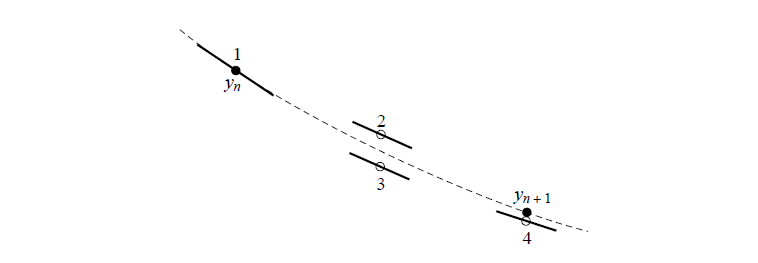
\includegraphics[scale=0.5]{rk4.png}
  \caption{\textit{Fourth-order Runge-Kutta method. In each step the derivative is evaluated four times:
once at the initial point, twice at trial midpoints, and once at a trial endpoint. From these derivatives the
final function value is calculated. }}
\end{figure}

\lstset{
  basicstyle=\small\ttfamily,
  frame=lrtb,
  numbers=left
}

Our implementation of the algorithm is shown below. f is a function that calculates and returns the derivative of the system state vector $A$, which contains the positions and velocities of all the objects.

\begin{lstlisting}[title={Function RK4}]
void Solver::RK4() {

    .....

    // vectors to use in the algorithm
    vec k1(6*n), k2(6*n), k3(6*n), k4(6*n);
 
    // time integration
    for (int i=0; i<N; i++) {

        k1 = f(A);
        k2 = f(A + k1*h2);
        k3 = f(A + k2*h2);
        k4 = f(A + k3*h);
        A += (h/6.0)*(k1 + 2*k2 + 2*k3 + k4);
        
        .....
    }
}
\end{lstlisting}



\subsubsection*{The Leap-Frog method}

The Leap-Frog scheme evaluates the positions and velocities at different time steps, in contrast to RK4. It is based on the Taylor expansion
\[
x(t+h) = x(t) + hx^{(1)}(t) + \frac{h^2}{2}x^{(2)}(t) + O(h^3)
\]
which can be rewritten as
\[
x(t+h) = x(t) + h \left( x^{(1)}(t) + \frac{h}{2}x^{(2)}(t) \right) + O(h^3)
\]
and if we also consider that
\[
x^{(1)}(t+h/2) = \left( x^{(1)}(t) + \frac{h}{2}x^{(2)}(t) \right) + O(h^2)
\]
we end up with
\[
x(t+h) = x(t) + hx^{(1)}(t+h/2) + O(h^3) \tag{1}
\]
which is the equation for finding the new position. This needs to be combined with
\[
x^{(1)}(t+h/2) = x^{(1)}(t-h/2) + hx^{(2)}(t) + O(h^2) \tag{2}
\]
thus the local truncation error goes like $h^3$ for the position and $h^2$ for the velocity.

As we can see the positions and velocities are evaluated at different time steps; only half-step velocities are computed. $x^{(1)}(t) = v(t)$ can be obtained explicitly if needed:
\[
x^{(1)}(t+h) = x^{(1)}(t+h/2) + \frac{h}{2}x^{(2)}(t) + O(h^2) \tag{3}
\]

The Leap-Frog algorithm can be summarized like this: We compute the velocity at $t+h/2$ with equation $(1)$ so that $x(t+h)$ can be obtained using $(2)$. The velocity at $t+h$ can be evaluated using equation $(3)$ if needed. This scheme requires that the accelerations $x^{(2)}(t) = a(t)$ are known, which in our case is provided by Newton's gravitational law.

\begin{figure}[H]
  \centering \includegraphics[scale=0.5]{leapfrog.png}
  \caption{\textit{Leap-Frog method. The positions and velocities are evaluated at different time steps.}}
\end{figure}

Our implementation of the Leap-Frog method is shown below.

 \begin{lstlisting}[title={Function Leap Frog}]
void Solver::LeapFrog() {

    double x, y, z, vx, vy, vz, ax, ay, az, ax_new, ay_new, az_new;

    vec vx_new(n);
    vec vy_new(n);
    vec vz_new(n);

    for(int j=0; j<N; j++) {

        Solver::SolveSystem(A);

        for(int i=0; i<n; i++) {

            int vi = values*i;

            x = A(vi);
            y = A(vi+1);
            z = A(vi+2);

            vx = dAdt(vi);
            vy = dAdt(vi+1);
            vz = dAdt(vi+2);

            ax = dAdt(vi+3); // ax(t)
            ay = dAdt(vi+4); // ay(t)
            az = dAdt(vi+5); // az(t)

            vx_new(i) = vx + (dt/2)*ax; // vx(t+dt/2)
            vy_new(i) = vy + (dt/2)*ay; // vy(t+dt/2)
            vz_new(i) = vz + (dt/2)*az; // vz(t+dt/2)

            A(vi) = x + dt*vx_new(i); // x(t+dt)
            A(vi+1) = y + dt*vy_new(i); // y(t+dt)
            A(vi+2) = z + dt*vz_new(i); // z(t+dt)
        }

        Solver::SolveSystem(A);

        for(int i=0; i<n; i++) {

            int vi = values*i;

            ax_new = dAdt(vi+3); // ax(t+dt)
            ay_new = dAdt(vi+4); // ay(t+dt)
            az_new = dAdt(vi+5); // az(t+dt)

            A(vi+3) = vx_new(i) + (dt/2)*ax_new; // vx(t+h)
            A(vi+4) = vy_new(i) + (dt/2)*ay_new; // vy(t+h)
            A(vi+5) = vz_new(i) + (dt/2)*az_new; // vz(t+h)
        }
    }
}
\end{lstlisting}

\subsection*{Implementing the methods}
In our program we have two classes: $Solver$ and $Planet$. $Solver$ does the majority of the tasks, including initialization of system parameters and objects. It also contains one solver function for each method (RK4 and Leap-Frog) in addition to functions calculating energies. $Planet$ creates an instance when called upon that contains information on the initial position, initial velocity and mass of each object.

\begin{lstlisting}[title={Making of instance}]
planet Earth = planet(1.0, 0.0, 0.0, 0.0, 2.*pi, 0.0, M_earth);
\end{lstlisting}

makes an instance Earth that contains the initial $x, y, z$ - positions and $v_x, v_y, v_z$ - velocities and the mass of Earth.

We then use these $Planet$ objects to create a vector $A$ that contains the initial positions, $(x,y,z)$, and the velocities, $(v_x,v_y,v_z)$, for all objects:

\[ A = \left( \begin{array}{c}
x - object \hspace*{0.5mm} 1\\
y - object \hspace*{0.5mm} 1\\
z - object \hspace*{0.5mm} 1 \\
vx - object \hspace*{0.5mm} 1\\
vy -object \hspace*{0.5mm} 1\\
vz - object \hspace*{0.5mm} 1 \\
x - object \hspace*{0.5mm} 2\\
... \\
vz - object \hspace*{0.5mm} n \end{array} \right)\]

$Solver$ also contains a function that finds the time derivative of these values, $dAdt$. The time derivative of the position is simply the velocity, and that value is already saved in $A$ and easy to obtain. To find the acceleration, that is the time derivative of the velocities, we use Newton's second law: For each object we sum the gravitational forces working on it from all the other objects according to Newton's gravitational law and divide by its mass.

To calculate the time propagation of the objects, we use RK4 and Leap-Frog as discussed above, both calculating the propagation forward in time starting from the given initial conditions.

Our program is built to solve the problem regardless of the dimension of $A$. Thus to change our system from the two-body problem to the $N$-body star cluster we need only change the initial system state vector $A$.

For the two-body system the initial conditions is quite straight forward

 \begin{lstlisting}[title={Initial conditions two-body system}]
 vec A = zeros(values*n);
 vec dAdt = zeros(values*n);
 vec M = zeros(n);

 planet Earth = planet(1.0, 0.0, 0.0, 0.0, 2.*pi, 0.0, M_earth);
 planet Sun = planet(0.0, 0.0, 0.0, 0.0, 0.0, 0.0, M_sun);
 planet B[n];

 B[0] = Earth;
 B[1] = Sun;

  // initial conditions

  for (int i=0; i<n; i++) {
        int j = values*i; // values = 2*dimensionality
       
        A(j) = B[i].x0; // x - position
        A(j+1) = B[i].y0; // y - position
        A(j+2) = B[i].z0; // z - position
        A(j+3) = B[i].vx; // vx - velocity
        A(j+4) = B[i].vy; // vy - velocity
        A(j+5) = B[i].vz; // vz - velocity

        M(i) = B[i].M;
        
   }
\end{lstlisting}
 
 
For the $N$-body system, however, the initial conditions are a bit more challenging. We wish to start with a uniform, random distribution of $N$ particles within a sphere of radius $R_0$. The initial velocities are easy: We will simulate what is called a "cold collapse", starting our particles with no initial velocity. The particle masses are randomly distributed by a Gaussian distribution around ten solar masses with a standard deviation of one solar mass.


\subsubsection*{Uniformly distributed random coordinates within a sphere and randomly distributed mass}

To find the coordinates of the particles we used the function $ran2$ that was available from the web page. It yields a random number between 0 and 1 when called upon with a negative seed. For our purpose we wish to convert these numbers into coordinates of uniformly distributed particles within a sphere of radius $R_0$.

To do this one can use spherical coordinates
\begin{equation}
\begin{split}
x &= r sin \theta cos \phi \\
y &= r sin \theta sin \phi \\
z &= r cos \theta
\end{split}
\end{equation}


where $ \theta \hspace{0.5mm} \epsilon \hspace{0.5mm} [0, \pi], \phi \hspace{0.5mm} \epsilon \hspace{0.5mm} [0, 2\pi], r \hspace{0.5mm} \epsilon \hspace{0.5mm} [0, R_0]$.
 
We then use the fact that the volume element should be the same for any coordinate system. We introduce three new variables with a uniform distribution between 0 and 1, and write the volume element in terms of these coordinates. We get
\[
r^2 sin \theta dr d \theta d \phi = Adudvdw
\]

where $A$ is just a constant and $u, v, w \hspace{0.5mm} \epsilon \hspace{0.5mm} [0,1]$. When separating the variables we get three equations

\[
r^2dr = adu \hspace{1cm}\mathrm{,}\hspace{1cm}
sin \theta = bdv \hspace{1cm}\mathrm{,}\hspace{1cm}
d \phi = cdw
\]

Integrating up we find that
\[
\phi = 2 \pi w \hspace{1cm}\mathrm{and}\hspace{1cm}
r = R_0 \sqrt[3]{u} \hspace{1cm}\mathrm{and}\hspace{1cm}
\theta = arccos(1-2v)
\]

After calculating these values it is easy to transform back to $(x,y,z)$-coordinates using the expressions for the spherical coordinates.

The mass of the objects should be randomly distributed by a Gaussian distribution around ten solar masses with a standard deviation of a solar mass. We used the function $gaussian_deviate$, which has a standard deviation $ \sigma = 1$ and is centred around zero. To get our wanted distribution with a standard deviation of $1$ and average of ten solar masses we used
$$ M = \sigma gaussian_deviate() + \mu $$
where $\sigma = 1$ and $\mu = 10$.

\begin{lstlisting}[title={Initial conditions for the N-body system}]
    for (int i=0; i<N; i++) {

        u = ran2(&idum);
        v = ran2(&idum);
        w = ran2(&idum);

        phi = 2*pi*w;
        r = R0*cbrt(u);
        theta = acos(1-2*v);

        x = r*sin(theta)*cos(phi);
        y = r*sin(theta)*sin(phi);
        z = r*cos(theta);

        int j = values*i;

        A(j) = x; // x - position
        A(j+1) = y; // y - position
        A(j+2) = z; // z - position
        A(j+3) = 0.0; // vx - velocity
        A(j+4) = 0.0; // vy - velocity
        A(j+5) = 0.0; // vz - velocity

        M(i) = sigma*gaussian_deviate(&idum) + mu;
    }
  
\end{lstlisting}

 
\subsection*{Results}

\subsubsection*{Comparing the algorithms}

We have tested our program for the two-body-problem Sun-Earth to find out which method that works best for this type of gravitational problem. We saw that with the right choice of time step both yields the wanted trajectory with the Earth in circular orbit around the Sun. See figure \ref{dt_0.002}.

\begin{figure}[H]
        \centering
        \begin{subfigure}[b]{0.6\textwidth}
                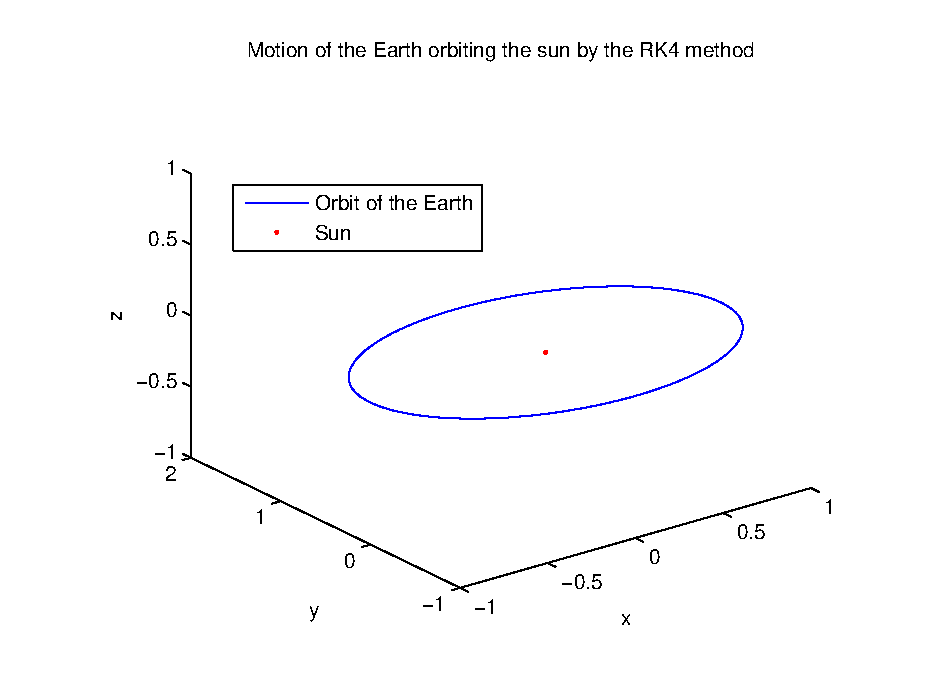
\includegraphics[width=\textwidth]{RK4_n_1000_t_2.pdf}
                \caption{Runge-Kutta method}
                \label{fig:RK4_dt_0.002}
        \end{subfigure}%
 )
        \begin{subfigure}[b]{0.6\textwidth}
                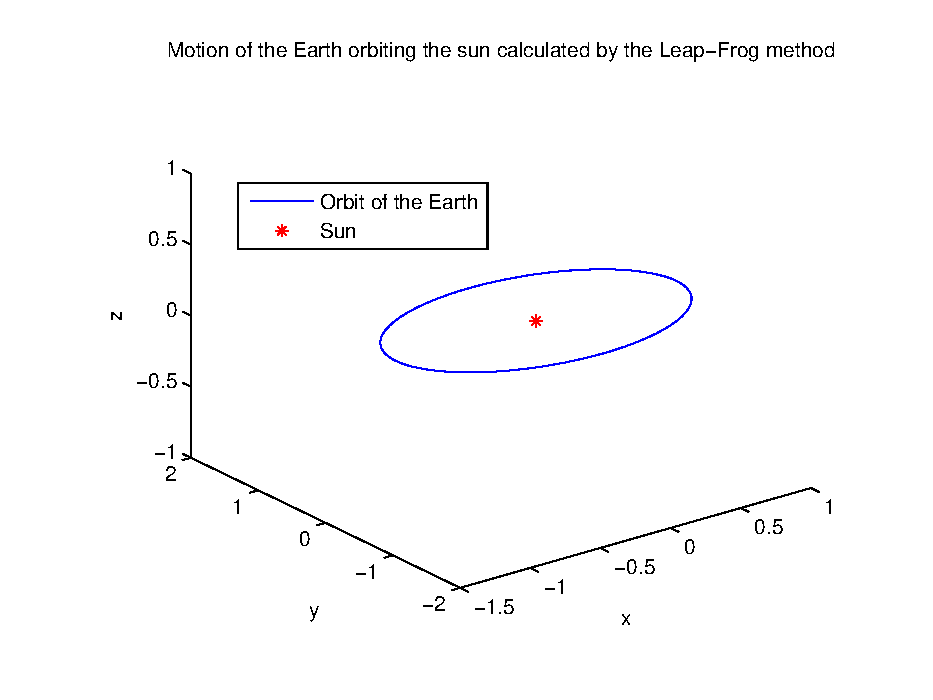
\includegraphics[width=\textwidth]{LF_n_1000_t_2.pdf}
                \caption{Leap-Frog method}
                \label{fig:LF_dt_0.002}
        \end{subfigure}
        \caption{Motion of the Earth orbiting the Sun calculated for two years with a time step $\Delta t = 0.002$}
\label{dt_0.002}
\end{figure}

These nice results are however not produced if the time step is large enough. From the figures \ref{dt_0.002} we see that time step $\Delta t = 0.002$ gives the wanted trajectory for both methods, while a time step of the order $\Delta t = 0.1$, \ref{dt0.1}, is unstable for both methods.

From the figures \ref{timestep} we see that the Leap-Frog method is less vulnerable to the wrong choice of time step than the Runge-Kutta solver. The radius should be constant at $1 AU$, but for large time steps we see that both methods get highly unstable. However, the Leap-Frog method tolerates a larger time step than the Runge-Kutta method before it gets unstable.


We see that for $\Delta t = 0.1$ the Runge-Kutta method gives a solution where the Earth starts spirals in towards the Sun. As the Earth gets too close to the Sun, a time step that was reasonable for more distant objects is far to large when we get close to the Sun. And thus we get the effect we see from figure \ref{dt0.1}; the Earth escapes from the Sun's gravitational field.

        
\begin{figure}[H]
        \centering
        \begin{subfigure}[b]{0.6\textwidth}
                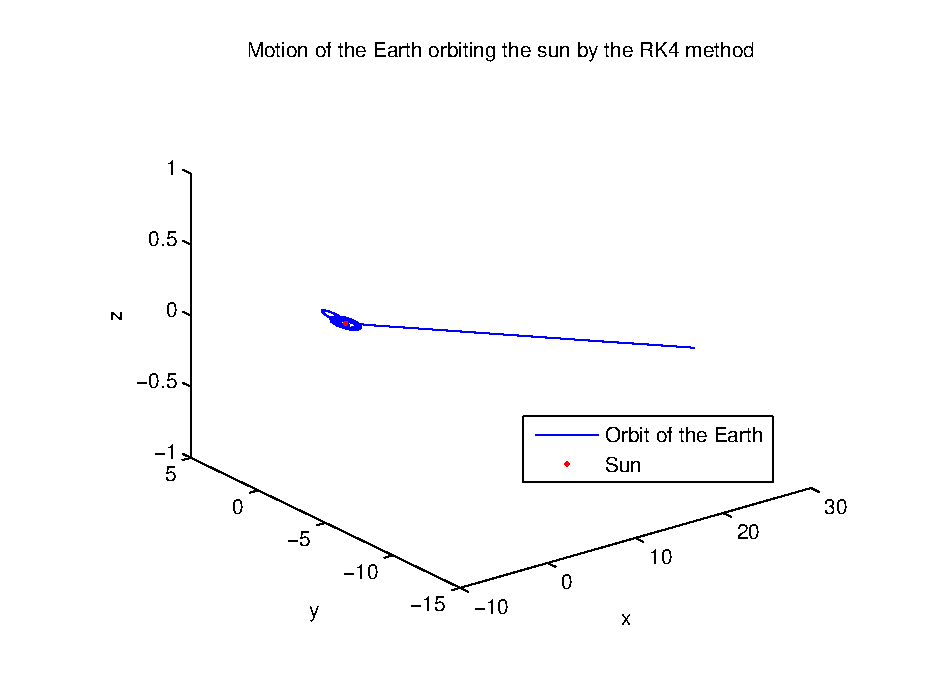
\includegraphics[width=\textwidth]{RK4_n_80_t_8.pdf}
                \caption{Runge-Kutta method}
                \label{fig:RK4_dt_0.1}
        \end{subfigure}%
        
        \begin{subfigure}[b]{0.6\textwidth}
                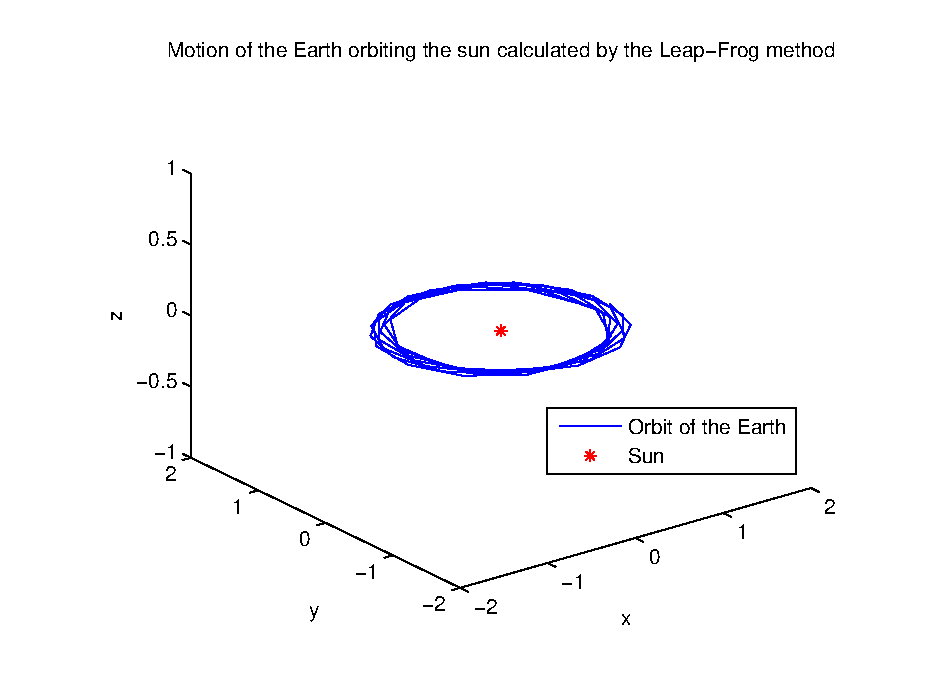
\includegraphics[width=\textwidth]{LF_n_80_t_8.pdf}
                \caption{Leap-Frog method}
                \label{fig:LF_dt_0.1}
        \end{subfigure}
        \caption{Motion of the Earth orbiting the Sun calculated for eigth years with a time step $\Delta t = 0.1$}
\label{dt0.1}
\end{figure}

\begin{figure}[H]
        \centering
        \begin{subfigure}[b]{0.6\textwidth}
                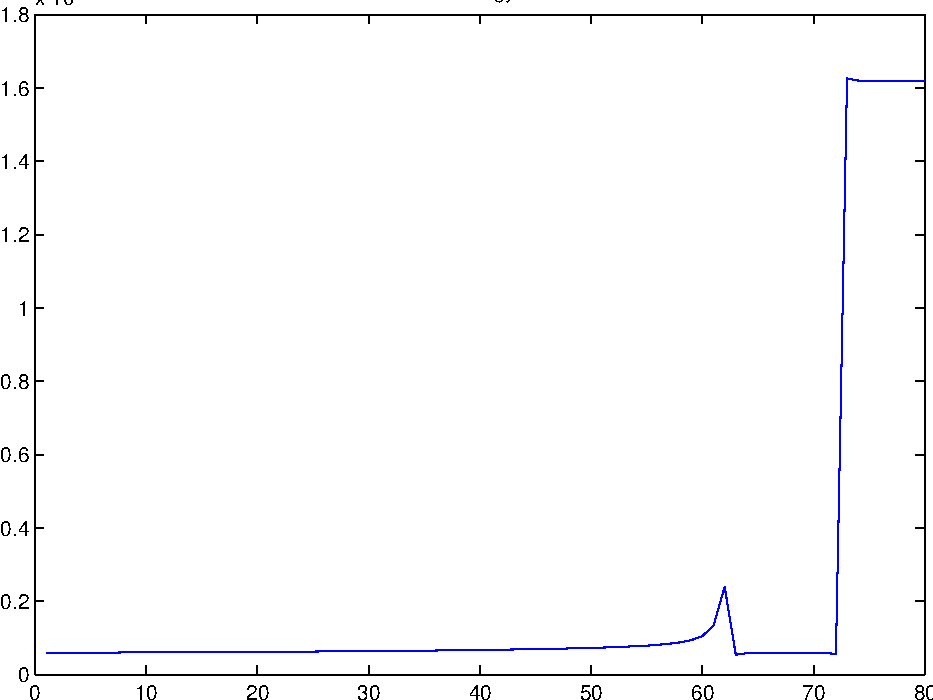
\includegraphics[width=\textwidth]{main_totE_rk4_dt_0_1.pdf}
                \caption{Runge-Kutta method absolute value of the total energy}
                \label{fig:RK4_dt_0.1}
        \end{subfigure}
       
        \begin{subfigure}[b]{0.8\textwidth}
                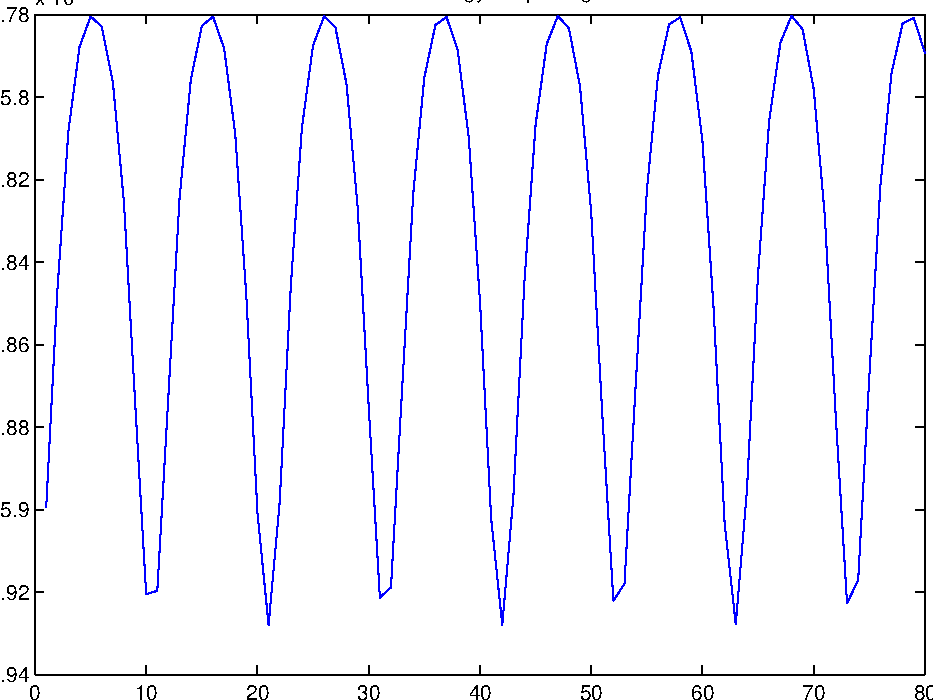
\includegraphics[width=\textwidth]{totE_main_lf_dt_0_1.pdf}
                \caption{Leap-Frog method}
                \label{fig:LF_dt_0.1}
        \end{subfigure}
        \caption{Energy for eigth years with a time step $\Delta t = 0.1$}
    
\end{figure}

        
\begin{figure}[H]
        \centering
        \begin{subfigure}[b]{0.6\textwidth}
                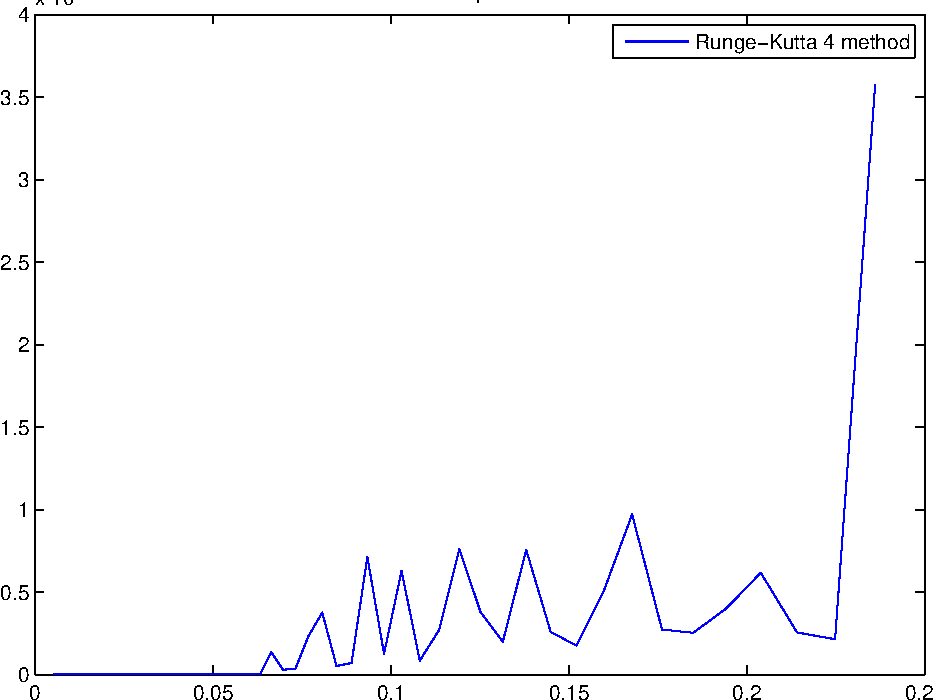
\includegraphics[width=\textwidth]{timestep_rk4.pdf}
                \caption{Plot over various time steps and the maximal radius for the Runge-Kutta solver}
                \label{fig:RK4_timestep}
        \end{subfigure}
        
        \begin{subfigure}[b]{0.8\textwidth}
                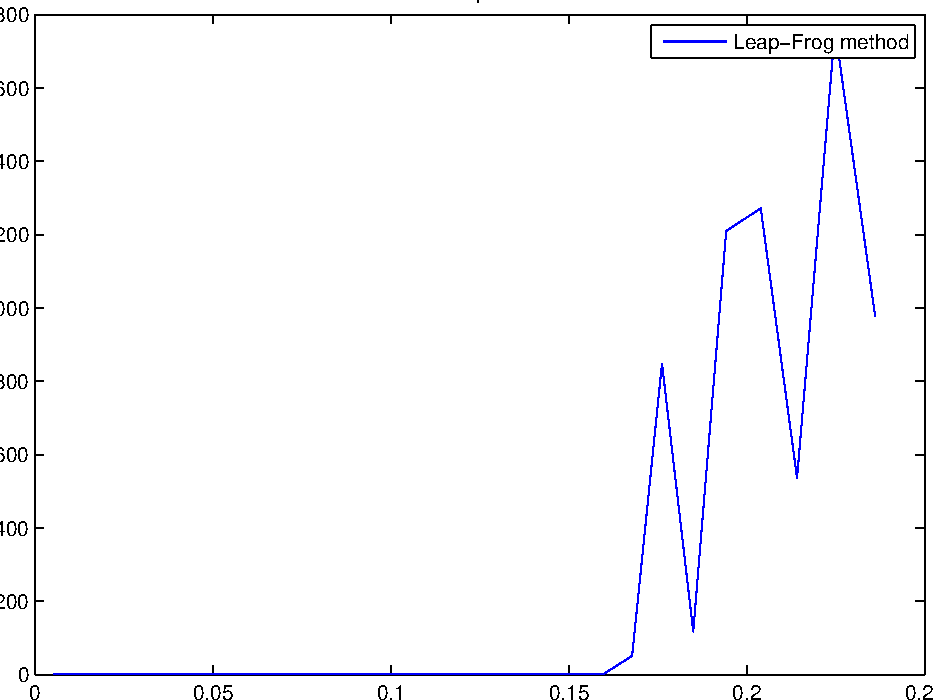
\includegraphics[scale=0.5]{timestep_LeapFrog.pdf}
                \caption{Plot over various time steps and the maximal radius for the Leap-Frog solver}
                \label{fig:LF_timestep}
        \end{subfigure}
        \label{timestep}
\end{figure}




\subsection*{Energy}

For the cluster simulation without the smoothing function, the particles is pulled towards the center of mass because of the gravitational force. When the particles get close together the acceleration, and thus the kinetic energy, increases a lot and the particles is spread out. See figure \ref{kin_pot_notsmooth}. The potential energy will increase as the particles is pulled together, but go to zero as the particles spreads out. 

\begin{figure}[H]
	\centering
        \begin{subfigure}[b]{0.6\textwidth}
        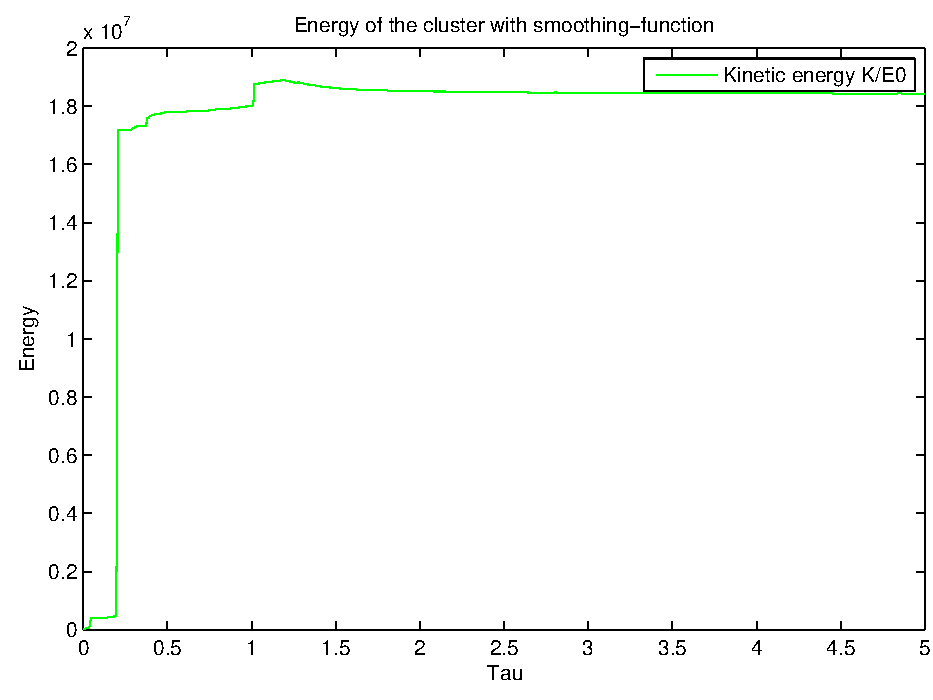
\includegraphics[scale=0.5]{kin_energy_without_smooth.pdf}
        \caption{\textit{Total kinetic energy for the cluster without smoothing function}}
        
		\end{subfigure}
		
		\begin{subfigure}[b]{0.6\textwidth}
        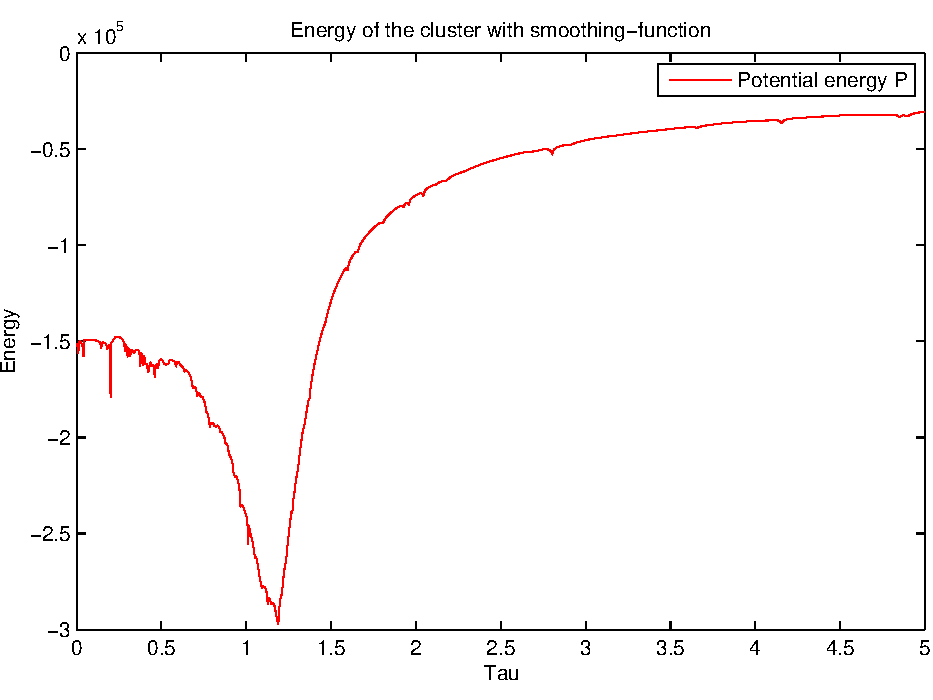
\includegraphics[scale=0.5]{pot_e_uten_smooth.pdf}
        \caption{\textit{Total potential energy for the cluster without smoothing function}}
		\end{subfigure}
		
		\begin{subfigure}[b]{0.6\textwidth}
        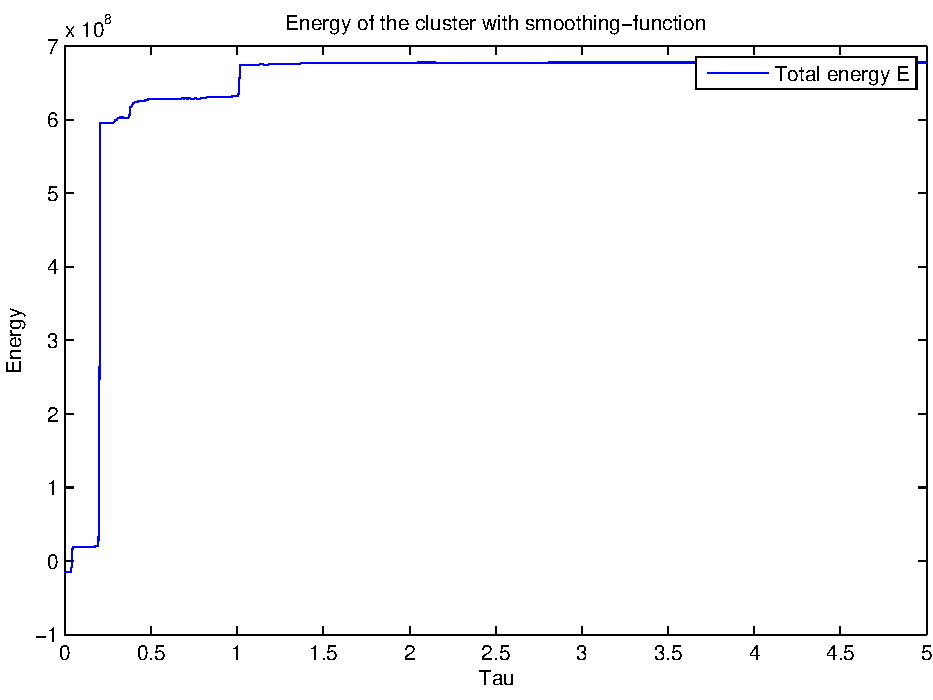
\includegraphics[scale=0.5]{tot_e_withouth_smooth.pdf}
        \caption{\textit{Total energy for the cluster without smoothing function}}
		\end{subfigure}
		
		\label{fig:kin_pot_notsmooth}        
\end{figure}



\begin{figure}[H]
	\centering
        \begin{subfigure}[b]{0.6\textwidth}
        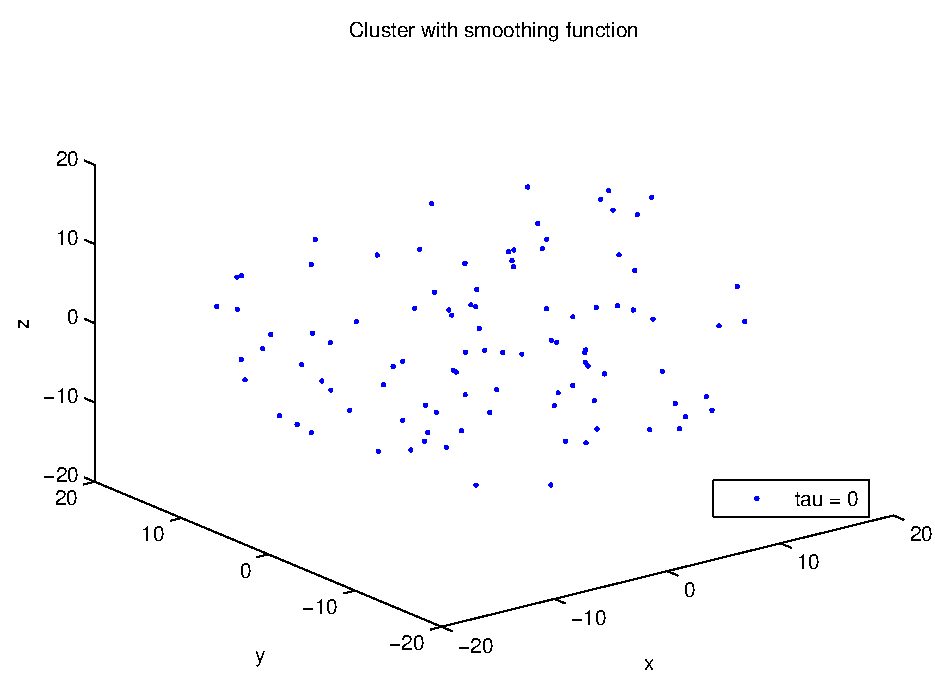
\includegraphics[scale=0.5]{CLUSTER_t0.pdf}
                
		\end{subfigure}
		
		\begin{subfigure}[b]{0.6\textwidth}
        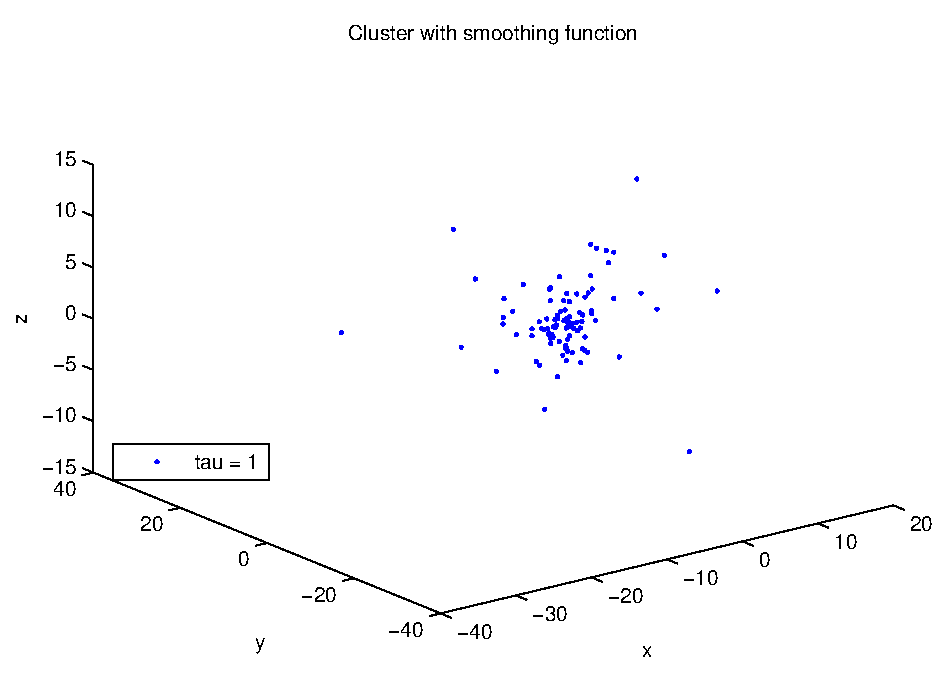
\includegraphics[scale=0.5]{CLUSTER_t1.pdf}
        \end{subfigure}
        
        \begin{subfigure}[b]{0.6\textwidth}
        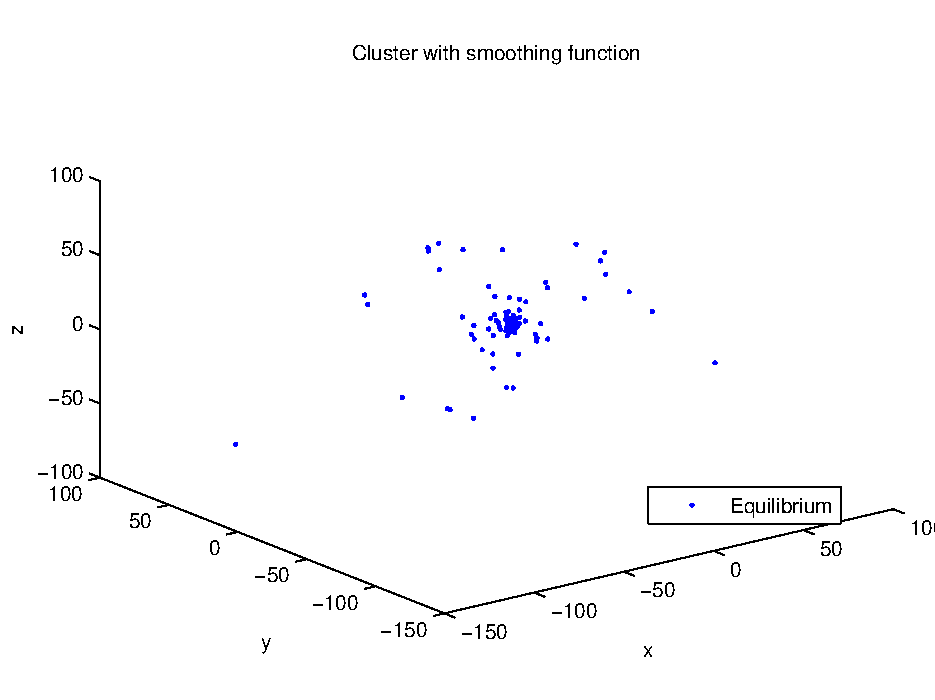
\includegraphics[scale=0.5]{CLUSTER_eq.pdf}
        \end{subfigure}
        
		\label{fig:cluster_smooth}        
		\caption{\textit{Simulation of cluster with smoothing function at $\tau = 0$, $\tau = 1$ and at equilibrium}}
\end{figure}

For the cluster system with the modified force we see from \ref{kin_pot} that the kinetic and the potential energy increases (that is the potential energy gets a larger negative value) towards the collapse at $\tau_{crunch}$. This we can also see from our animation of the cluster. At first the particles, that initially has no velocity, are dragged towards the center by the gravitational force from the other particles. Thus the particles are accelerated and the kinetic energy increases. As the particles come closer together, the gravitational force between them gets stronger as well and the potential energy increases. As we reach the time of the collapse, at $\tau_{crunch}$, many of the particles are ejected. Disregarding the energies of these particles, we find that both the kinetic and potential energy decreases and stabilizes as the system reaches an equilibrium. Both the kinetic and potential energy will fluctuate some, but stays approximately constant.    

\begin{figure}[H]
	\centering
        \begin{subfigure}[b]{0.6\textwidth}
        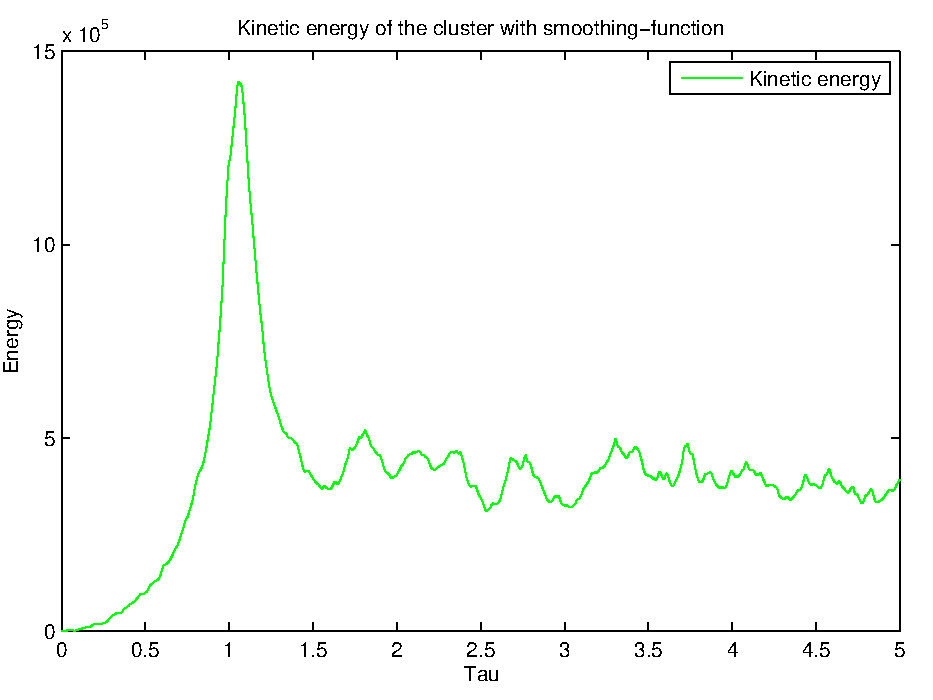
\includegraphics[scale=0.5]{kine_n1000t5.pdf}
        \caption{\textit{Total kinetic energy for the cluster with smoothing function}}
        
		\end{subfigure}
		
		\begin{subfigure}[b]{0.6\textwidth}
        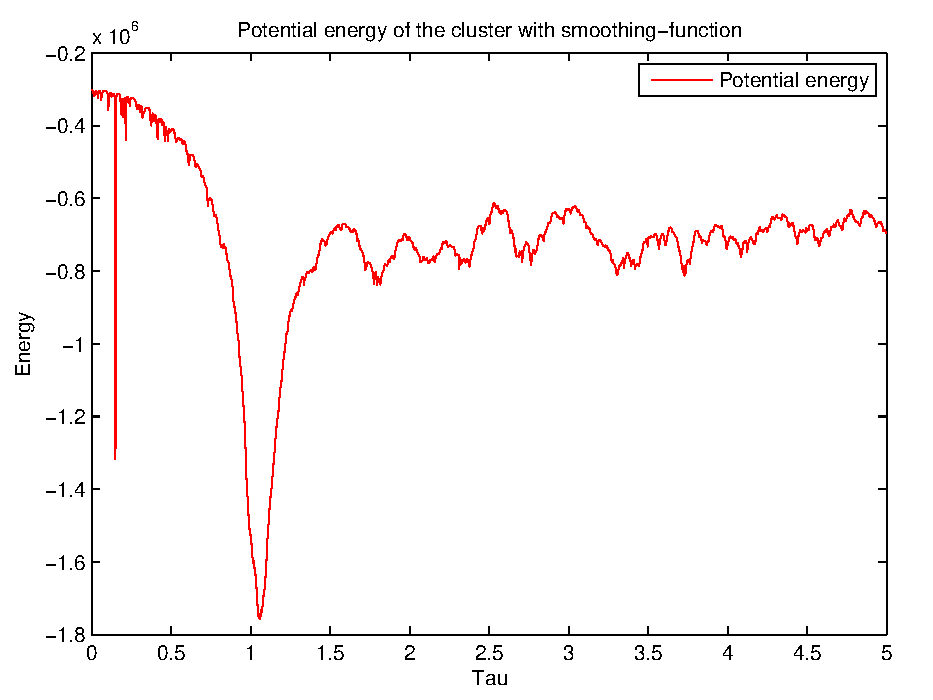
\includegraphics[scale=0.5]{pote_n1000t5.pdf}
        \caption{\textit{Total potential energy for the Cluster with smoothing function}}
		\end{subfigure}
		\label{fig:kin_pot}        
\end{figure}



\begin{figure}
        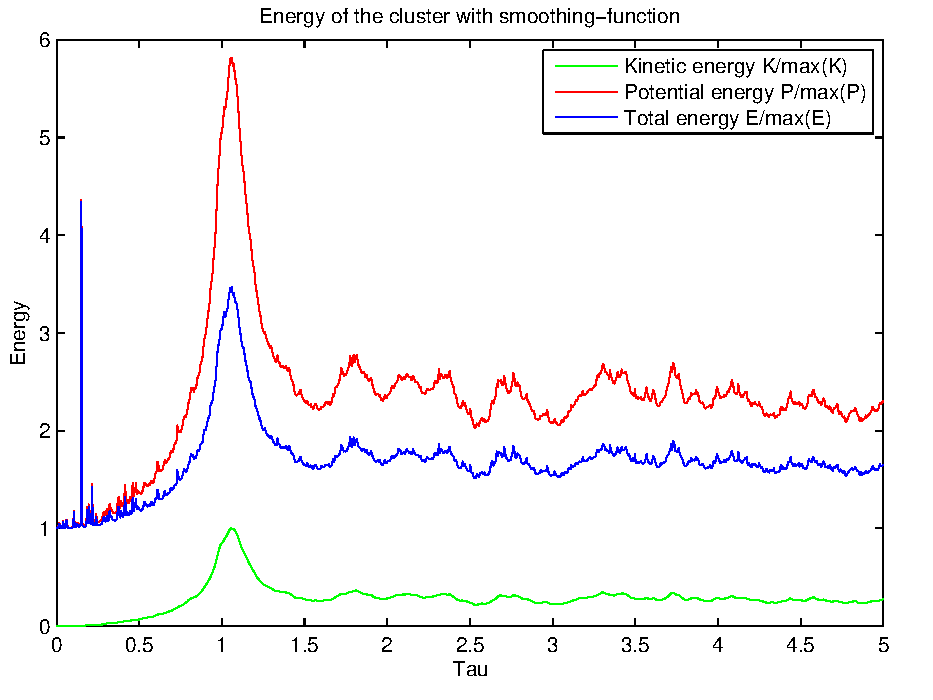
\includegraphics[scale=0.5]{energy_n1000t5_N100.pdf}
        \caption{\textit{Total kinetic energy for the cluster with smoothing function}}
        \label{fig:totE}
\end{figure}

To test if the energies are in consistency with the virial theorem 
\[
2\langle K\rangle = -\langle V \rangle
\]

we calculated the total potential energy divided by the total kinetic energy for a late time step where the system is in equilibrium. We found that this value was approximately $-2$, as it should be.

\subsubsection*{Radial density}

\begin{figure}[H]
	\centering
        \begin{subfigure}[b]{0.6\textwidth}
        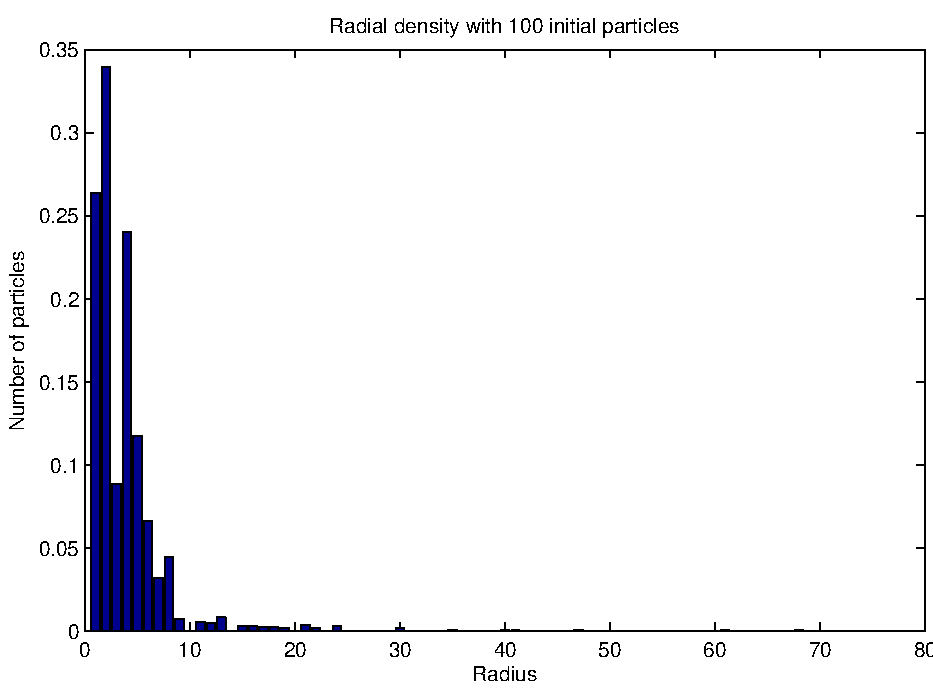
\includegraphics[scale=0.5]{Radial_densit_100.pdf}
        \caption{\textit{N = 100}}
        
		\end{subfigure}
		
		\begin{subfigure}[b]{0.6\textwidth}
        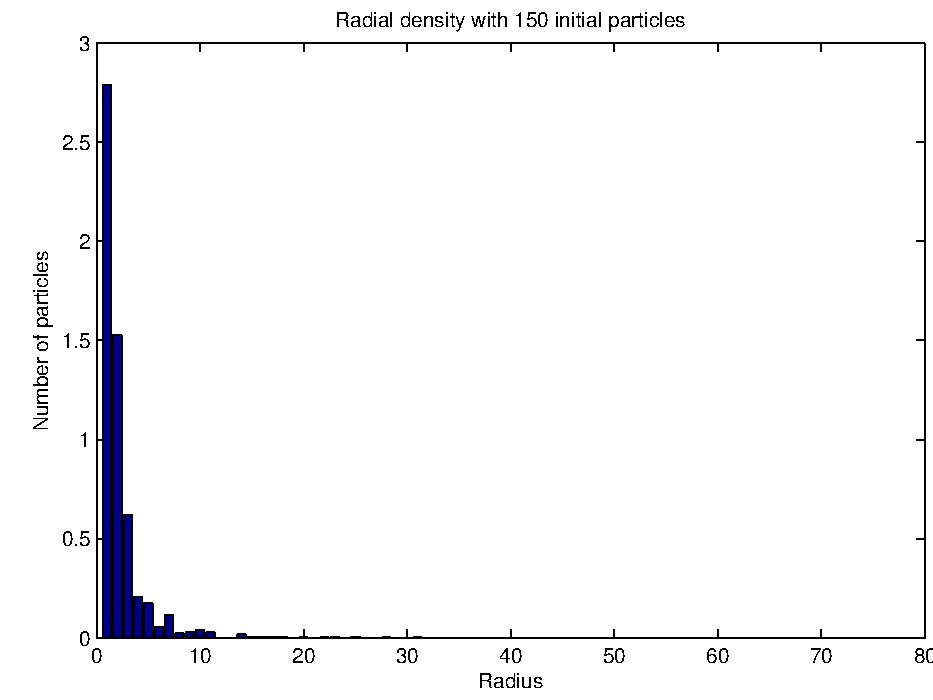
\includegraphics[scale=0.5]{Radial_density_150.pdf}
        \caption{\textit{N = 150}}
		\end{subfigure}
		
		\begin{subfigure}[b]{0.6\textwidth}
        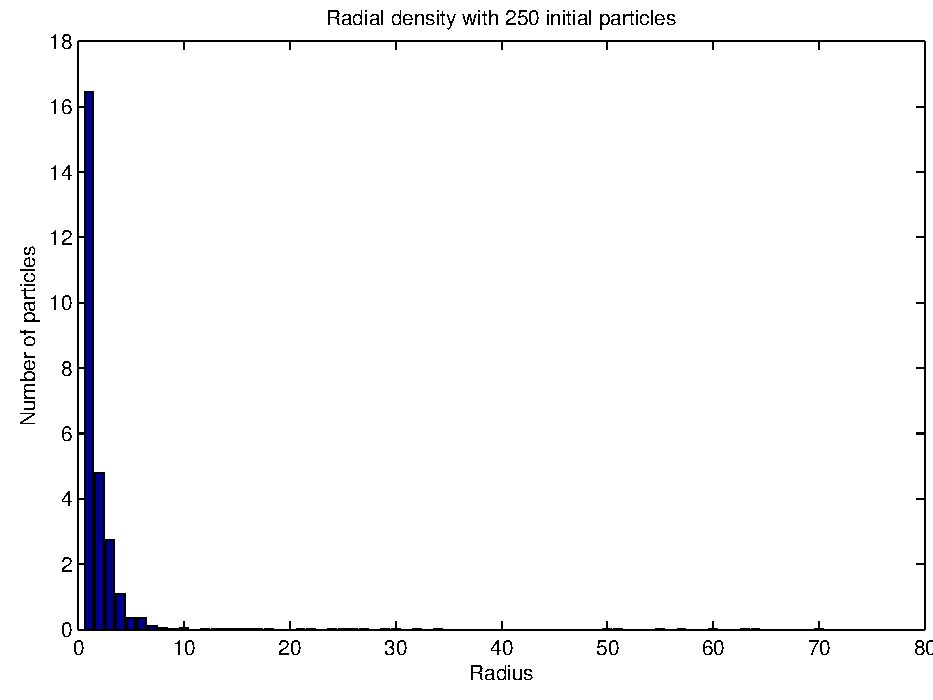
\includegraphics[scale=0.5]{radial_density_250.pdf}
        \caption{\textit{N = 250}}
		\end{subfigure}
		
		\begin{subfigure}[b]{0.6\textwidth}
        \includegraphics[scale=0.5]{radial_density_500.pdf}
        \caption{\textit{N = 500}}
		\end{subfigure}
		
		\label{fig:radial density}       
				 
\end{figure}

\begin{tabular}{ l c r }
 N & Average distance & Standard deviation \\ 
 \hline 
  100 & 23 ly & 22 ly \\
  150 &  13 ly & 15 ly \\
  250 & 12 ly & 16 ly \\
  500 & 8 ly & 13 ly \\
\end{tabular}

\subsection*{Conclusion}
 

\end{document}

    

